\section{Convolutional Neural Network}

Convolutional Neural Networks (CNNs) are a type of deep learning architecture designed to automatically and efficiently extract spatial features from images.
CNNs are composed of several core building blocks, each serving a specific function in the feature extraction process. 
The main components of a CNN include:
\begin{itemize}
    \item Convolutional layers.
    \item Nonlinearities (activation functions, such as ReLU).
    \item Pooling layers (e.g., max pooling for subsampling).
\end{itemize}
These layers work together to progressively transform an input image into more abstract and useful representations for the task at hand, such as classification or object detection.

\paragraph*{Architecture}
The architecture of a CNN typically involves stacking multiple blocks of these layers.
As the input image passes through the network, it is transformed through a sequence of increasingly complex feature maps or volumes:
\begin{itemize}
    \item As the depth of the network increases, the height and width of the image representation shrink.
    \item Each layer takes a 3D input volume (height, width, and channels) and outputs a transformed volume.
\end{itemize}
\begin{figure}[H]
    \centering
    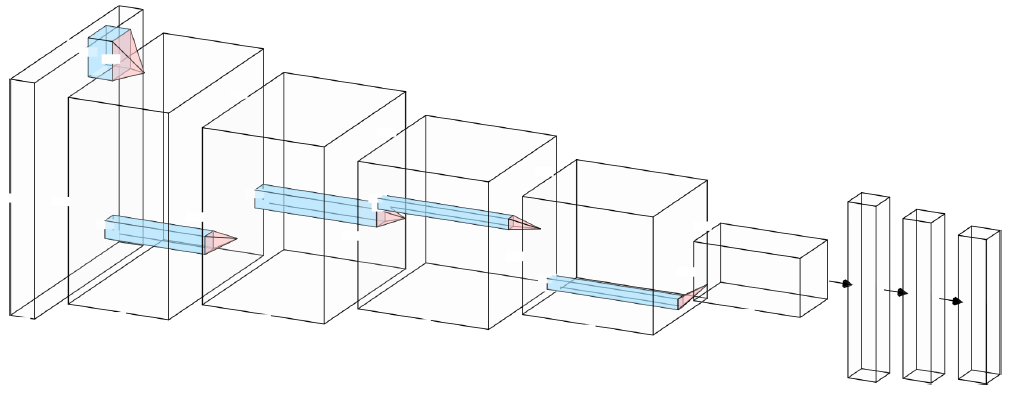
\includegraphics[width=0.5\linewidth]{images/cnn.png}
    \caption{Convolutional Neural Network architecture}
\end{figure}

\subsection{Convolutional layers}
The core operation of a CNN is the convolution. In a convolutional layer, small regions of the input (known as receptive fields) are processed using filters (or kernels), which are learned during training. 
The input image, represented as a volume with dimensions height $h$, width $w$, and three channels for RGB, is transformed by these filters.

Each convolutional layer typically outputs a set of activation maps or "feature maps," each corresponding to a different filter. 
As the network grows deeper, the number of channels (i.e., the depth of the feature maps) increases, while the spatial dimensions (height and width) decrease.

For a filter $w$ applied over the input image, the output at a given location $(r, c)$ and channel $l$ is computed as:
\[a(r,c,l)=\sum_{(u,v)\in U,k=1,\dots,C}w^l(u,v,k)x(r+u,c+v,k)+b^l\qquad\forall(r,c),l=1,\dots,N_F\]
Here: 
\begin{itemize}
    \item $(r,c)$ refers to a spatial location in the output activation map $a$.
    \item $l$ denotes the output channel index (or filter). 
    \item $U$ represents the spatial neighborhood (receptive field) of the convolution filter. 
    \item $C$ is the number of input channels (e.g., 3 for an RGB image).
\end{itemize}
A filter is characterized by:
\begin{itemize}
    \item \textit{Spatial size}: a small neighborhood $U$ (e.g., 3x3 or 5x5) over which the convolution is applied.
    \item \textit{Depth}: the same as the number of channels in the input volume, ensuring that the filter processes the full input depth.
\end{itemize}
The total number of parameters in a convolutional layer is determined by the size of the filters and the number of filters. 
Specifically:
\[\text{Total parameters }=(h_r\cdot h_c\cdot C)\dot N_F+N_F\]
Here, $h_r$ and $h_c$ are the height and width of the filter, $C$ is the input depth, and $N_F$ is the number of filters.

\paragraph*{Key characteristics}
The key characteristics of the convolutional layers in a Convolutional Neural Network are: 
\begin{itemize}
    \item \textit{Local processing}: convolutions operate over a small spatial neighborhood $U$, meaning the filter looks at localized regions of the image at a time.
    \item \textit{Channel-wise} processing: Filters span the entire depth of the input volume to capture information across all channels.
    \item \textit{Output volume}: the result of applying a filter is a slice of the output volume, often referred to as an activation map. 
        Each filter produces a different slice of this volume.
\end{itemize}

\paragraph*{Summary}
Convolutional layers are defined by a set of learned filters.
Filters perform linear combinations of the input over localized spatial regions.
Filters are small in spatial extent, but span the full depth of the input volume.
The depth of each output activation map corresponds to the number of filters used.

As the input passes through successive convolutional layers, its representation becomes increasingly abstract, capturing high-level features such as shapes, textures, and patterns. 
This allows CNNs to efficiently and automatically learn features directly from raw image data, significantly improving performance on tasks like image classification.

\subsection{Activation layer}
ctivation layers introduce nonlinearities into the network, which is essential for the CNN to model complex patterns. 
Without nonlinear activation functions, a CNN would be equivalent to a linear classifier, limiting its capacity to capture intricate relationships in the data.

Activation functions are applied element-wise, meaning they operate on each individual value in the feature map (or volume) independently. 
Importantly, they do not change the size or dimensions of the volume but modify the values within it.

The most used activation functions are: 
\begin{itemize}
    \item \textit{ReLU} (Rectified Linear Unit): the ReLU activation function is defined as:
        \[f(x)=\max(0,x)\]
        It introduces nonlinearity by thresholding the input values—any negative values are set to zero, while positive values remain unchanged. 
        ReLU has become the most widely used activation function in deep neural networks, particularly since its adoption in the AlexNet architecture. 
        Its simplicity and effectiveness have made it the default choice for most CNNs.
        ReLU accelerates convergence during training by mitigating the vanishing gradient problem that often affects sigmoid and tanh functions.

        One issue with ReLU is the dying neuron problem, where some neurons can become permanently inactive if they consistently output zero. 
        This occurs when their weights are updated in such a way that they never activate again.
    \item \textit{Leaky ReLU}: to address the dying neuron problem, Leaky ReLU introduces a small slope for negative values, allowing a small gradient to flow even when the input is negative:
        \[T(x)=\begin{cases}
            x \qquad\text{if } x \geq 0 \\
            0.01x \qquad\text{otherwise}
        \end{cases}\]
        This modification helps prevent neurons from becoming inactive, ensuring they can still contribute to learning even when their inputs are negative.
    \item \textit{Tanh} (Hyperbolic Tangent): the tanh activation function has a range of $(-1, 1)$ and is continuous and differentiable:
        \[f(x)=\tanh(x)\]
        Tanh is similar to the sigmoid function but is symmetric around zero, which can make optimization easier as it centers the data. 
        However, like sigmoid, tanh can still suffer from the vanishing gradient problem when used in deep networks.
    \item \textit{Sigmoid}: the sigmoid activation function is given by:
        \[f(x)=\dfrac{1}{1+e^{-x}}\]
        It outputs values between $0$ and $1$, making it useful for binary classification tasks. 
        However, sigmoid has largely fallen out of favor in deep CNN architectures due to the vanishing gradient problem, where gradients become very small during backpropagation, slowing down learning in deeper layers.
\end{itemize}
ReLU and Leaky ReLU are by far the most popular activation functions in CNNs due to their simplicity, computational efficiency, and performance in deep networks.
Functions like sigmoid and tanh are more commonly used in traditional multi-layer perceptron (MLP) architectures and certain specialized layers like output layers, where specific output ranges are needed.
By introducing nonlinearities, activation functions allow CNNs to learn complex, non-linear mappings from input to output, which is crucial for tasks like image classification and object detection.

\subsection{Pooling layer}
Pooling layers are used to reduce the spatial dimensions (height and width) of the input volume, while preserving the most important information. 
This downsampling helps in making the network more computationally efficient and less prone to overfitting, as it reduces the number of parameters in the network.

\paragraph*{Max pooling}
ooling layers operate independently on each depth slice (or channel) of the input volume. 
The most common type of pooling is Max Pooling, which selects the maximum value within a defined region of the input.
For example, in a 2x2 pooling window, Max Pooling considers each 2x2 region of the input, and only retains the maximum value from that region. 
This results in a significant reduction of the spatial size—typically discarding 75\% of the input data (since the 2x2 window compresses 4 values into 1).
Max Pooling effectively downscales the image while keeping the most prominent features. 
This helps retain important characteristics like edges or corners, which are crucial for tasks like image classification.

\paragraph*{Strides}
The stride determines how much the pooling window moves across the input volume. 
Typically, the stride is equal to the size of the pooling window (e.g., for 2x2 pooling, a stride of 2 is commonly used). 
This halves the height and width of the input volume.

If not explicitly specified, Max Pooling usually has a stride equal to the pooling size (e.g., stride = 2 for 2x2 pooling), reducing the spatial dimensions of the image by a factor of 2.
If strides is unitary, is possible to use a stride of 1, where the pooling operation moves by one pixel at a time. 
This doesn't reduce the spatial dimensions but instead applies the pooling operation over overlapping regions. 
This is typically combined with nonlinear pooling (like max pooling) and is useful when downsampling isn't needed but feature extraction is still required.

\subsection{Final architecture}
\begin{figure}[H]
    \centering
    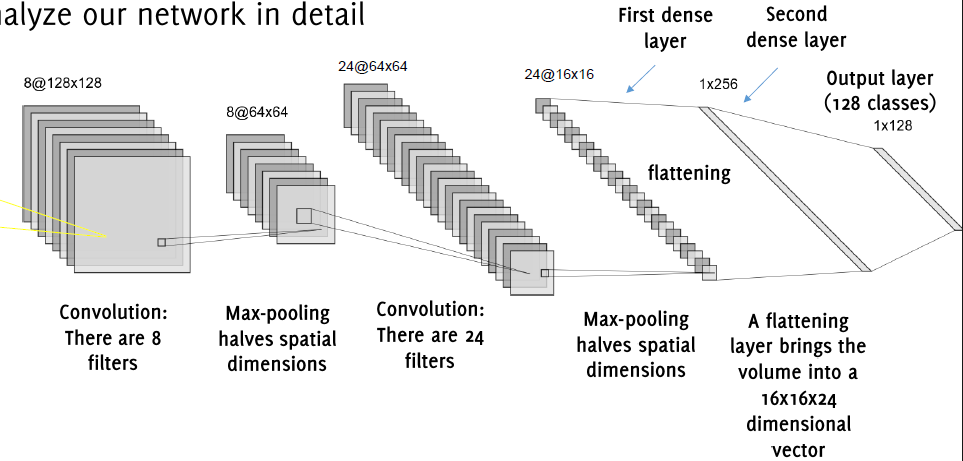
\includegraphics[width=0.5\linewidth]{images/cnn1.png}
    \caption{Convolutional Neural Network complete architecture}
\end{figure}
As we progress through the layers of a Convolutional Neural Network (CNN), the number of feature maps (or channels) increases, while the spatial dimensions of the image (height and width) decrease. 
This allows the network to capture more abstract and high-level features, while reducing the computational complexity.

Once the spatial dimensions of the feature maps are sufficiently reduced, the output is flattened into a 1D vector. 
This vector is then fed into a traditional fully connected (Dense) neural network, where each neuron is connected to every neuron in the previous layer. 
At this point, the spatial structure is lost, and the network focuses on combining the high-level features learned during the convolutional and pooling stages for the final classification.

Flattening converts the 3D feature maps into a single vector, enabling their input into fully connected layers.
This step is essential as it transforms the hierarchical features extracted by the convolutional layers into a format suitable for classification.

The fully connected layers follow the flattened vector and are responsible for classification. 
The final fully connected layer typically has an output size equal to the number of target classes, providing a score (or probability) for each class.
Dense layers are called fully connected because each output neuron is connected to every input neuron.
The final layer often applies a softmax activation function to convert the raw output scores into probabilities for each class.

\paragraph*{Learning representation}
Throughout the CNN, convolutional filters are learned to detect patterns relevant to the classification task. 
This includes applying operations such as ReLU (thresholding) and max pooling (downsampling) to progressively simplify the feature maps.

The architecture typically involves stacking many convolutional, activation, and pooling layers to learn meaningful representations from the data. 
This depth allows the network to capture low-level features in the initial layers, and more complex patterns (e.g., shapes, objects) in the deeper layers.

\subsection{Convolutional and dense layers}
Convolution is fundamentally a linear operation. 
When an input image is unrolled into a vector, the convolutional weights can be conceptualized as the weights of a dense layer.
Both convolutional and dense layers can be represented as linear operators, expressed mathematically as:
\[\mathbf{a}=\mathbf{Wx}+\mathbf{b}\]

\paragraph*{Dense layers}
In dense layers, the weight matrix is fully populated, meaning each input neuron is connected to every output neuron through distinct weights. 
This results in a comprehensive interaction among neurons.

\paragraph*{Convolutional layers}
Conversely, convolutional layers exhibit sparse connectivity. 
Here, each output neuron is influenced only by a subset of input neurons, reflecting the localized nature of convolution.
As a result, most entries in the weight matrix are zero. 
The convolutional operation spans all channels of the input, leading to a circular structure within the weight matrix.

In convolutional layers, weights are shared across the entire output channel. 
The same filter is applied to compute the output for multiple positions, effectively shifting the filter across the input. 
This mechanism results in several output neurons sharing the same weights and bias values, which are constant across blocks corresponding to the filters.

\paragraph*{Spatial invariance}
A defining characteristic of Convolutional Neural Networks (CNNs) is spatial invariance. 
All neurons within the same slice of a feature map utilize the same weights and biases, significantly reducing the total number of parameters in the network. 
The underlying assumption here is that if a feature is useful for computation at one spatial position, it should also be useful at different positions.

Every convolutional layer can be mathematically implemented as a fully connected layer that performs equivalent computations.
The weight matrix for a convolutional layer would be large, with the number of rows equal to the number of output neurons and the number of columns equal to the number of input neurons. 
This matrix is predominantly sparse, filled mostly with zeros, except for specific blocks where local connectivity is established. 
Moreover, many weights within these blocks are identical due to parameter sharing.
Interestingly, the converse interpretation is also valid and offers insightful perspectives on their functional equivalence.

\subsection{Receptive field}
The concept of the receptive field is fundamental in deep Convolutional Neural Networks. 
Unlike fully connected networks, where each output is influenced by the entire input, each output in a CNN is determined by a specific localized region of the input. 
This localized region is referred to as the receptive field for that output.

As the network depth increases, the receptive field expands. 
This expansion occurs through various mechanisms, including convolutions, strides, and max pooling, which collectively contribute to the widening of the receptive field. 
Typically, the receptive field is defined concerning the final output unit of the network relative to the input; however, this definition is equally applicable to intermediate feature maps.

In deeper layers, neurons are influenced by larger patches of the input. 
Notably, convolutions alone are sufficient to increase the receptive field, eliminating the necessity for max pooling.

As we progress deeper into the network:
\begin{itemize}
    \item The spatial resolution of the feature maps diminishes.
    \item The number of feature maps generally increases.
\end{itemize}
At these deeper layers, the focus shifts to detecting higher-level patterns, allowing for a degree of insensitivity to their exact spatial location. 
This is essential, as higher-level patterns are often more abundant and informative than low-level details.